%%%%%%%%%%%%%%%%%%%%%%%%%%%%%%%%%%%%%%%%%%%%%%%%%%%%%%%%%%%%%%%%%%%%%%%%%%%%%%%%%%%%
\documentclass{article}
\usepackage[margin=1in]{geometry}
\usepackage{amsmath,amsthm,amssymb,amsfonts, fancyhdr, color, comment, graphicx, environ}
\usepackage{xcolor}
\usepackage[utf8]{inputenc}
\usepackage[T1]{fontenc}
\usepackage[italian]{babel}
\usepackage{mdframed}
\usepackage{minted}
\usepackage{xcolor}
\usepackage[shortlabels]{enumitem}
\usepackage{indentfirst}
\usepackage{hyperref}
% Define emphasis
\DeclareTextFontCommand{\emph}{\bfseries\em}
\hypersetup{
    colorlinks=true,
    linkcolor=blue,
    filecolor=magenta,
    urlcolor=blue,
}

\definecolor{LightGray}{gray}{0.9}

\pagestyle{fancy}
% Define problem environment
\newenvironment{problem}[2][Domanda]
    { \begin{mdframed}[backgroundcolor=gray!20] \textbf{#1 #2} \\}
    {  \end{mdframed}}

% Define solution environment
\newenvironment{solution}
    {\textit{Risposta:}}
    {}

\renewcommand{\qed}{\quad\qedsymbol}

% Prevent line break in inline mode
\binoppenalty=\maxdimen
\relpenalty=\maxdimen

%%%%%%%%%%%%%%%%%%%%%%%%%%%%%%%%%%%%%%%%%%%%%
% Document information (author, course, date)
\lhead{Karina Chichifoi }
\rhead{\today}
\chead{\textbf{Ingegneria del software Q\&A}}
%%%%%%%%%%%%%%%%%%%%%%%%%%%%%%%%%%%%%%%%%%%%%
% Define huge title
\makeatletter
\newcommand\HUGE{\@setfontsize\Huge{30}{40}}
\makeatother
\begin{document}
% TITLEPAGE
\begin{titlepage}
	\centering
	\large
	A cura di Karina Chichifoi - Ultima revisione: \today

	\noindent\rule{15cm}{0.2pt}

	\vspace{1.5cm}

	\HUGE
	\textbf{Ingegneria del Software Q\&A}

	\vspace{17cm}

	\normalsize
	\url{https://github.com/TryKatChup/IngegneriaSoftware_QA}

	\clearpage
\end{titlepage}
% Premessa
\renewcommand{\abstractname}{}
\begin{abstract}
	\section*{Premessa}
	Ho scritto questo file in modo da facilitare lo studio e il superamento dell'esame di Ingegneria del Software.
	Tuttavia è consigliato integrare questo materiale con le slide del professore Marco Patella, disponibili sulla piattaforma \textit{Insegnamenti Online}.

	\section*{Contribuire alla guida}

	Se ritieni di poter migliorare la guida, oppure se sono state aggiunte altre domande al di fuori di questo file, o se hai trovato un errore, visita la repository GitHub ed apri una \textit{issue}, oppure inviami un messaggio. Ogni contributo è ben accetto :)

	\vspace{4mm}
	Link Repository: \url{https://github.com/TryKatChup/IngegneriaSoftware_QA}

	\vspace{5mm}

	\begin{figure}[htb!]
		\centering
		
\includegraphics[width=4cm]{qrcode.png}
		\caption{QR Code alla repository di GitHub}
	\end{figure}
\end{abstract}
\newpage
\section{Modulo 1}
\begin{problem}{1.1}
Come viene implementata l'ereditarietà multipla?
\end{problem}
\begin{solution}
\end{solution}
\begin{problem}{1.2}
Si esegua una classificazione del polimorfismo secondo Cardelli-Wegner e si mostri l'implementazione del polimorfismo per inclusione.
\end{problem}
\begin{solution}
\end{solution}
\begin{problem}{1.3}
Procedimento di compilazione ed esecuzione del codice all'interno del framework .NET tramite il CLR.
\end{problem}
\begin{solution}
\end{solution}

\begin{problem}{1.4}
Tipi di dati in .NET
\end{problem}
\begin{solution}
\end{solution}


\begin{problem}{1.5}
Differenza tra tipi valore e tipi riferimento in .NET
\end{problem}
\begin{solution}
\end{solution}


\begin{problem}{1.6}
Garbage Collector in C\#
\end{problem}
\begin{solution}
\end{solution}


\begin{problem}{1.7}
Passaggio dei parametri in C\#
\end{problem}
\begin{solution}
\end{solution}




\begin{problem}{1.8}
Concetto di delegato in C\#
\end{problem}
\begin{solution}
\end{solution}


\begin{problem}{1.9}
Metaprogrammazione e riflessione in C\#
\end{problem}
\begin{solution}
\end{solution}


\begin{problem}{1.10}
Spiegare i quattro bad design (fragilità, immobilità, rigidità, viscosità)
\end{problem}
\begin{solution}
La qualità del design risulta fondamentale per rendere un programma:
\begin{itemize}
	\item Maggiormente affidabile
	\item Maggiormente efficiente
	\item Maggiormente manutenibile
	\item Maggiormente economico
\end{itemize}
Esistono quattro principi che peggiorano la qualità del software:
\begin{enumerate}
	\item \textbf{Rigidità del software}: rende complesse le modifiche al software, in quanto una piccola modifica influenza gran parte del programma, a causa di modifiche a cascata su moduli dipendenti tra loro.
	\newline Una conseguenza di questo principio è la quantità di tempo necessaria a gestire una modifica del software.
	\item \textbf{Fragilità del software}: responsabile del malfunzionamento del software di fronte a una modifica di quest'ultimo; il software risulta difficile da mantenere, in quanto per ogni correzione è presente un rischio maggiore di guasto.
	\item \textbf{Immobilità del software}: rende il software inutilizzabile da parti dello stesso progetto o da altri progetti; ciò avviene quando un modulo software è fortemente dipendente da altri moduli.
	\newline Di conseguenza occorre scrivere nuovo software, anziché riutilizzarlo.
	\item \textbf{Viscosità del software}: questo principio favorisce l'utilizzo di \textit{hack}, ovvero soluzioni funzionanti, ma che snaturano il design, in quanto non seguono le \textit{best practice}.
	\newline
	La viscosità è maggiormente presente nel caso in cui utilizzo di hack risulta molto più semplice di una soluzione che preserva la progettazione iniziale.
	\newline
	Esistono due categorie di viscosità:
	\begin{itemize}
		\item \textbf{Viscosità del design}: l'utilizzo di metodi che rispettano il design risulta più complesso che utilizzare hack.
		\item \textbf{Viscosità dell'ambiente}: l'ambiente di sviluppo è lento e inefficiente: si possono avere tempi di compilazione molto lunghi, il sistema di controllo del codice sorgente richiede ore per la registrazione di pochi file.
	\end{itemize}
\end{enumerate}
I motivi di una progettazione non corretta sono dovuti a:
\begin{itemize}
	\item Incapacità dei progettisti nel seguire le \textit{best practice}
	\item Limiti imposti dall'esterno, in termini di tempo e risorse
	\item Pratiche obsolete
	\item Evoluzione del progetto: in seguito a cambiamenti dei requisiti e modifiche al software, non si ha più la manutenibilità del progetto originario
\end{itemize}
\end{solution}


\begin{problem}{1.11}
Principio di singola responsabilità con almeno un esempio
\end{problem}
\begin{solution}
Il principio di singola responsabilità afferma che ogni elemento di un programma (classe, metodo, variabile) deve avere un'unica responsabilità, interamente gestita dall'elemento stesso.
Tutti i servizi offerti dall'elemento stesso dovrebbero essere allineati a tale responsabilità.
\newline
Una responsabilità risulta un motivo per cambiare, e ogni classe o modulo deve avere un solo motivo per cambiare.
\newline
Un esempio che rispetta il principio di singola responsabilità è un metodo \textit{setter}, in quanto la sua unica responsabilità è quella di impostare il valore di una variabile appartenente a una classe.
\end{solution}


\begin{problem}{1.12}
Principio di inversione delle dipendenze con almeno un esempio
\end{problem}
\begin{solution}
Il principio di inversione delle dipendenze prevede che i moduli di alto livello (i \textit{clienti}) non debbano dipendere dai moduli di basso livello(ovvero i \textit{fornitori dei servizi} ). Entrambi devono dipendere da \textit{astrazioni}.
\newline
Il motivo della precedente affermazione è dovuto alla presenza di codice e della logica implementativa nei moduli di basso livello. Nel caso in cui i moduli di alto livello dovessero dipendere da moduli di basso livello si avrebbe:
\begin{itemize}
	\item \textbf{Rigidità}: per ogni modifica occorre intervenire su un numero elevato di moduli
	\item \textbf{Fragilità}: per ogni modifica verrebbero introdotti errori nel sistema
	\item \textbf{Immobilità}: non è possibile riutilizzare il codice, in quanto i moduli di alto livello non si riuscirebbero a separarare da quelli di basso livello.
\end{itemize}
Con il principio di inversione delle dipendenze si eviterebbero i problemi sopra elencati, in quanto le astrazioni possiedono poco codice e sono poco soggetti a modifiche; inoltre è presente una separazione tra moduli astratti e moduli concreti, che permette modifiche limitate al modulo concreto interessato (poichè nessuno dipende da questi moduli).
Dato che i dettagli del sistema sono stati isolati da un muro di astrazioni stabili, pertanto:
\begin{itemize}
	\item I cambiamenti non possono più propagarsi (\textit{design for change})
	\item I singoli moduli sono maggiormente riusabili (\textit{design for resue})
\end{itemize}
\end{solution}


\begin{problem}{1.13}
Principio di segregazione delle interfacce con almeno un esempio
\end{problem}
\begin{solution}
Questo principio prevede che un cliente non debba dipendere dai metodi che non usa, e che quindi è preferibile avere più interfacce specifiche, anzichè una sola interfaccia con più funzioni (\textit{fat interface}).
\newline
Nel caso di utilizzo delle \textit{fat interfaces} sarà più difficile mantenere il sistema, in quanto è rappresentato da un unico blocco; pertanto occorre creare interfacce specifiche per ogni cliente.
\newline
Un esempio di mancato utilizzo di principio di segregazione delle interfacce è la creazione, da parte di Xerox (fondatore di \textit{Ethernet}), di una stampante che aveva diverse funzionalità, tra cui mandare fax e pinzare fogli. Le modifiche al software, sebbene piccole, risultavano difficili, in quanto tutte le diverse funzioni eseguite dalla stampante multi-uso erano implementate all'interno di una sola classe.
\end{solution}


\begin{problem}{1.14}
Principio aperto/chiuso con almeno un esempio
\end{problem}
\begin{solution}
Il principio aperto/chiuso prevede un sistema aperto a estensioni software, ma chiuso a modifiche.
\newline
Per realizzare questo principio vengono utilizzate classi astratte e interfacce; nel caso in cui si vogliano aggiungere nuove funzionalità sarà necessario, anzichè modificare il codice, implementare una nuova classe concreta che implementa le astrazioni.
\newline
Questo approccio consente una maggiore modularità del sistema e stabilità, in quanto non si modificano componenti definite precedentemente e non si introducono eventuali errori dovuti alle modifiche.
\end{solution}


\begin{problem}{1.15}
Principio di sostituibilità di Liskov con almeno un esempio
\end{problem}
\begin{solution}
Il principio di sostituibilità di Liskov definisce il rapporto tra una classe e le relative sottoclassi.
Esistono due versioni di questo principio:
\begin{itemize}
	\item \textbf{Versione debole}: a ogni riferimento della classe base (classe padre) deve essere associata l'istanza della sottoclasse (classe figlia)
	\item \textbf{Versione forte}: ogni programma che utilizza istanze della classe base non percepisce variazioni logiche nell'utilizzo delle istanze delle relative sottoclassi.
\end{itemize}
Per essere più specifici, occorre introdurre due concetti definiti dal \textit{design by contract}:
\begin{itemize}
	\item \textbf{Precondizioni}: requisiti minimi che devono essere soddisfatti dal chiamante, affinchè il metodo invocato possa essere eseguito correttamente
	\item \textbf{Postcondizioni}: requisiti soddisfatti dal metodo chiamato, nel caso di esecuzione corretta
\end{itemize}
Per ogni metodo re-implementato dalla sottoclasse:
\begin{itemize}
	\item Le precondizioni devono essere ugualmente o meno stringenti
	\item Le postcondizioni devono essere ugualmente o più stringenti
	\item La semantica della classe base deve essere conservata
	\item Non è possibile aggiungere vincoli alla classe base
\end{itemize}
Ad esempio, data la classe \texttt{Uccello} dotata del metodo \texttt{vola()} si hanno i due seguenti scenari:
\begin{itemize}
	\item la sottoclasse \texttt{Pinguino}, che eredita da \texttt{Uccello}, presenta una violazione del principio di sostituibilità di Liskov, in quanto l'utilizzo del metodo \texttt{vola()} deve essere ridefinito, senza mantenere la semantica (ad esempio sollevando un'eccezione, dato che un pinguino non può volare).
	\item la sottoclasse \texttt{Piccione}, che eredita da \texttt{Uccello}, non presenta una violazione del principio di sostituibilità di Liskov, in quanto la semantica del metodo \texttt{vola()} viene rispettata.
\end{itemize}
\end{solution}


\begin{problem}{1.16}
Principi per l'architettura dei package
\end{problem}
\begin{solution}
\end{solution}


\begin{problem}{1.17}
Pattern Singleton con esempi
\end{problem}
\begin{solution}
Il pattern Singleton prevede che una classe abbia una sola istanza; chiunque può accedervi attraverso l'unica istanza citata.
Una classe che implementa il pattern Singleton è strutturata nel sequente modo:
\begin{minted}
[
frame=lines,
framesep=2mm,
baselinestretch=1.2,
bgcolor=LightGray,
fontsize=\footnotesize,
linenos
]
{java}
public class Singleton {

   private static Singleton istance = null; // riferimento all' istanza

   private Singleton() {} // costruttore

   public static Singleton getIstance() {
	if (istance == null)
	   istance = new Singleton();
    return istance;
   }

   public void metodo() { ... }

}

\end{minted}
Il costruttore è privato, in quanto assicura che viene creata al più un'istanza della classe \texttt{Singleton}.
Il metodo statico \texttt{getInstance()} controlla se è già esistente un'istanza della classe: in caso affermativo restituisce l'istanza creata in precedenza, altrimenti crea una nuova istanza.
\newline
Una classe con soli membri statici non rappresenta un'alternativa al pattern Singleton, in quanto non permette di creare istanze personalizzate in base al contesto; non permette inoltre di utilizzare un numero arbitrario di interfacce.
\newline
Un esempio di utilizzo del pattern Singleton è l'accesso a un database, in quanto si vuole garantire atomicità.
\begin{figure}[h]
    \centering
    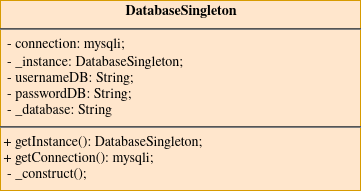
\includegraphics[scale=0.5]{./immagini/DatabaseSingleton.png}
      \label{logo}
  \end{figure}
\end{solution}

\newpage
\begin{problem}{1.18}
Pattern Observer con esempi
\end{problem}
\begin{solution}
Il pattern Observer viene utilizzato nel caso in cui il cambiamento di un oggetto preveda un aggiornamento degli altri oggetti (\textit{observer}).
È previsto un accoppiamento uno a molti: l'oggetto che vuole ricevere un aggiornamento (\texttt{Observer}) si iscrive a \texttt{Subject}, che prevede un metodo \texttt{notify()}, il quale notifica tutti gli Observer dell'aggiornamento effettuato.
Il diagramma UML previsto per il pattern Observer è il seguente:
\end{solution}


\begin{problem}{1.19}
Pattern Strategy con esempi
\end{problem}
\begin{solution}

\end{solution}


\begin{problem}{1.20}
Pattern Adapter con esempi
\end{problem}
\begin{solution}
\end{solution}

\begin{problem}{1.21}
Pattern Decorator con esempi
\end{problem}
\begin{solution}
\end{solution}

\begin{problem}{1.22}
Pattern Composite con esempi
\end{problem}
\begin{solution}
\end{solution}

\begin{problem}{1.23}
Modello LMU nei VCS con vantaggi e svantaggi
\end{problem}
\begin{solution}
\end{solution}
\newpage
\section{Modulo 2}
\begin{problem}{2.1}
Spiegare il modello a cascata e le sue criticità.
\end{problem}
\begin{solution}
Il modello a cascata (waterfall model) è un modello di processo di sviluppo software che prevede fasi sequenziali distinte tra loro:
\begin{itemize}
	\item Studio di fattibilità
	\item Analisi dei requisiti
	\item Analisi del problema
	\item Progettazione
	\item Implementazione
	\item Collaudo
	\item Manutenzione
\end{itemize}
Ciascuna fase di sviluppo deve essere svolta in maniera esaustiva, prima di passare alla successiva, in modo da non tornare più indietro.
Per questo modello è importante definire:
\begin{itemize}
	\item \textbf{Semilavorati}: consistono in documentazione di tipo cartaceo, codice dei singoli moduli, sistema nel suo complesso.\newline
	Vengono prodotti da una fase, e utilizzati dalla fase successiva; in questo modo viene garantito un controllo della qualità del lavoro eseguito in ogni fase.
	\item \textbf{Date}: stabiliscono una scadenza entro la quale devono essere prodotti i semilavorati, in modo da tracciare il progresso del lavoro (workflow).
\end{itemize}
L'efficacia del modello a cascata è determinata dai seguenti fattori:
\begin{itemize}
	\item \textbf{Immutabilità dell'analisi}: i clienti sono in grado di esprimere tutte le loro richieste sin da subito, pertanto nella fase iniziale del progetto si possono definire tutte le funzionalità che il software deve eseguire
	\item \textbf{Immutabilità del progetto}: progettare l'intero sistema prima di avere scritto codice risulta possibile
\end{itemize}
Un importante vantaggio di questo approccio risulta essere un maggiore controllo dell'andamento del progetto; tuttavia la rigidità di questo modello rappresenta un grosso svantaggio, in quanto:
\begin{itemize}
	\item Man mano che il sistema prende forma le sue specifiche cambiano in continuazione, così come la visione che i clienti hanno del sistema
	\item Spesso, per avere prestazioni migliori, occorre revisionare il progetto.
\end{itemize}
Per risolvere parzialmente i problemi sopra citati si è introdotto un modello a cascata con forme limitate di retroazione a un livello.
Una possibile soluzione al problema consiste nel realizzare un prototipo che, una volta terminato il compito, viene abbandonato (\textit{throw-away prototyping}); successivamente viene costruito il sistema reale rispettando il modello a cascata.
\newline
Tuttavia quest'ultimo approccio risulta talmente dispensioso da eliminare i vantaggi economici del modello a cascata.
\end{solution}


\begin{problem}{2.2}
Spiegare il modello a cascata e il modello iterativo
\end{problem}
\begin{solution}
Per il modello a cascata si veda la domanda 2.1.
\newline
Il modello iterativo prevede un numero elevato di passi nel ciclo di sviluppo che iteramente aumentano il livello di dettaglio del sistema.
Uno svantaggio di questo modello è che non può essere utilizzato nella realizzazione dei progetti significativi.
Un esempio di processo di sviluppo che utilizza il modello iterativo è \textit{Rational Unified Process} (RUP).
\end{solution}


\begin{problem}{2.3}
Illustrare RUP
\end{problem}
\begin{solution}
Il \textit{Rational Unified Process} (RUP) rappresenta un modello di processo software \textbf{iterativo} (si veda domanda 2.2) e \textbf{ibrido} (contiene elementi di tutti i modelli di processo generici) pensato per software di grandi dimensioni.
\newline
Esistono tre aspetti importanti del processo di sviluppo:
\begin{itemize}
	\item \textbf{Prospettiva dinamica}: mostra l'evoluzione del modello nel tempo. È composta da 4 fasi:
	\begin{enumerate}
		\item \textbf{Avvio}: lo scopo di questa fase è di delineare il \textit{business case}, ovvero comprendere il tipo di mercato a cui si rivolge, le entità esterne (persone e sistemi) che interagiscono con il sistema.
		\newline
		Durante la fase di avvio si utilizzano modelli di caso d'uso e si effettua una valutazione dei rischi.
		\item \textbf{Elaborazione}: questa fase definisce la struttura complessiva del sistema; comprende l'analisi del dominio e una prima fase di progettazione dell'architettura.
		\newline
		Occorre soddisfase alcuni criteri, tra i quali:
		\begin{itemize}
			\item Modello dei casi d'uso completo all' 80\%
			\item Descrizione dell'architettura del sistema
			\item Sviluppo dell'architettura del sistema
			\item Sviluppo di un'architettura eseguibile adatta agli use case significativi
			\item Revisione dei business case e dei rischi
			\item Pianificazione del progetto complessivo
		\end{itemize}
		\textbf{Nota bene:} al termine di questa fase modificare il progetto risulterà più difficile e dannoso.
		\item \textbf{Costruzione}: durante questa fase avviene la progettazione, la programmazione e il collaudo del sistema.
		Lo sviluppo delle diverse parti del sistema avviene in parallelo; successivamente vengono integrate.
		\newline
		Al termine di questa fase il sistema software dovrebbe essere funzionante e la relativa documentazione dovrebbe risultare pronta.
		\item \textbf{Transizione}: il sistema passa dall'ambiente di sviluppo a quello dell'utente finale. Quest'ultimo viene istruito nell'utilizzo del sistema, e si effettua \textit{beta testing} del sistema a scopo di verifica e validazione.
	\end{enumerate}
	\item \textbf{Prospettiva statica}: si focalizza sulle attività di produzione del software, note come \textit{workflow}; la descrizione di questi ultimi è orientata ai modelli associati a UML.
	Esistono sei workflow principali:
	\begin{enumerate}
		\item \textbf{Modellazione delle attività aziendali}: i processi aziendali vengono modellati, sfruttando il \textit{business case}
		\item \textbf{Requisiti}: vengono sviluppati i casi d'uso per la stesura dei requisiti; avviene l'identificazione degli attori che interagiscono con il sistema
		\item \textbf{Analisi e progetto}: attraverso l'utilizzo dei modelli architetturali e sequenziali degli oggetti e delle componenti viene creato e documentato un \textit{modello di progetto}
		\item \textbf{Implementazione}: i componenti vengono implementati; grazie alla generazione automatica del codice a partire dai modelli precedentemente definiti
		\item \textbf{Test}: vengono testati i sottocomponenti e il sistema finale
		\item \textbf{Rilascio}: il prodotto viene distribuito agli utenti
	\end{enumerate}
	Oltre ai 6 workflow principali vengono definiti 3 workflow di supporto:
	\begin{enumerate}
		\item \textbf{Gestione della configurazione e delle modifiche}: gestisce i cambiamenti del sistema
		\item \textbf{Gestione del progetto}: gestisce lo sviluppo del sistema
		\item \textbf{Ambiente}: fornisce agli sviluppatori degli strumenti adeguati
	\end{enumerate}
	\item \textbf{Prospettiva pratica}: suggerisce le \textit{buone prassi} da seguire nello sviluppo dei sistemi.
	\newline
	Esistono sei fasi fondamentali:
	\begin{enumerate}
		\item \textbf{Sviluppare ciclicamente il software}: pianificare (??) e consegnare le funzioni aventi la priorità più alta
		\item \textbf{Gestire i requisiti}: documentare ogni richiesta esplicita del cliente e ogni cambiamento effettuato, analizzandone l'impatto
		\item \textbf{Usare architetture basate sui componenti}: strutturare l'architettura del sistema in più componenti
		\item \textbf{Usare modelli visivi del software}: utilizzare grafici UML per la rappresentazione statica e dinamica del software
		\item \textbf{Verificare la qualità del software}: assicurarsi che vengano raggiunti gli standard di qualità previsti dall'organizzazione
		\item \textbf{Controllare le modifiche del software}: utilizzare strumenti e pratiche che permettono di gestire modifiche al software
	\end{enumerate}
\end{itemize}

\end{solution}

\begin{problem}{2.4}
Tipologie di analisi dei requisiti (in particolare quelli della sicurezza)
\end{problem}
\begin{solution}

\end{solution}

\begin{problem}{2.5}
Si illustri brevemente il ciclo di vita della valutazione del rischio
\end{problem}
\begin{solution}
L'analisi del rischio si occupa di bilanciare eventuali perdite, dovute ad attacchi informatici, con i costi richiesti per assicurare la protezione dei beni.
\newline
Un'importante componente dell'analisi del rischio è la valutazione del rischio, composta da pù fasi:
\begin{itemize}
	\item \textbf{Valutazione preliminare del rischio}: determina i requisiti di sicurezza dell'intero sistema
	\item \textbf{Ciclo di vita della valutazione del rischio}: avviene parallelamente al ciclo di vita dello sviluppo del software.
	\newline
	In questa fase occorre conoscere l'architettura del sistema e l'organizzazione dei dati.
	\newline
	La scelta della piattaforma e del middleware è stata già effettuata, così come la strategia di sviluppo del sistema; ciò consente di conoscere meglio cosa è necessario proteggere e quali sono le possibili vulnerabilità del sistema, alcune delle quali determinate da scelte progettuali precedenti.
	\newline
	In questa fase vengono effettuate l'\textit{identificazione} e la \textit{valutazione} della vulnerabilità, ovvero quali beni hanno la maggiore probabilità di essere colpiti.
	\newline
	Il risultato della valutazione del rischio è un insieme di decisioni ingegneristiche che influenzano la progettazione o l'implementazione del sistema.
\end{itemize}
\end{solution}

\begin{problem}{2.6}
Principali categorie di requisiti per la sicurezza
\end{problem}
\begin{solution}
Lo scopo dei requisiti di sicurezza è di definire quali comportamenti risultano inaccettabili per il sistema, senza definire le funzionalità richieste al sistema.
I requisiti di sicurezza specificano il contesto, i beni da proteggere e il valore che questi ultimi hanno per l'organizzazione.
\newline
Le categorie dei requisiti per la sicurezza sono:
\begin{itemize}
	\item \textbf{Requisiti di identificazione}: specificano se un sistema deve eseguire l'identificazione dei clienti, prima di una qualsiasi interazione con loro
	\item \textbf{Requisiti di autenticazione}: specificano le modalità di autenticazione degli utenti
	\item \textbf{Requisiti di autorizzazione}: specificano i permessi e i privilegi che gli utenti possiedono una volta identificati
	\item \textbf{Requisiti di immunità}: specificano i meccanismi di difesa che il sistema deve adottare per difendersi da eventuali malware
	\item \textbf{Requisiti di integrità}: specificano come evitare le corruzioni dei dati
	\item \textbf{Requisiti di scoperta delle intrusioni}: specificano quali meccanismi vengono adottati per la rilevazione degli attacchi
	\item \textbf{Requisiti di non-ripudiazione}: specificano che una parte interessata in una transazione non può negare il proprio coinvolgimento
	\item \textbf{Requisiti di riservatezza}: specificano come deve essere mantenuta la riservatezza delle informazioni
	\item \textbf{Requisiti di controllo della protezione}: specificano come deve essere controllato e verificato l'utilizzo del sistema
	\item \textbf{Requisiti di protezione della manutenzione del sistema}: specificano come un' applicazione può evitare modifiche autorizzate, nel caso in cui accidentalmente vengano annullati i meccanismi di protezione
\end{itemize}
\end{solution}


\begin{problem}{2.7}
Commentare eventuali errori di un diagramma UML
\end{problem}
\begin{solution}

\end{solution}


\begin{problem}{2.8}
Linee guida di progettazione nella sicurezza
\end{problem}
\begin{solution}

\end{solution}

\begin{problem}{2.9}
White box e black box testing
\end{problem}
\begin{solution}

\end{solution}

\begin{problem}{2.10}
Capacità di sopravvivenza del sistema
\end{problem}
\begin{solution}

\end{solution}

\end{document}
